%========================%
% Beginning of Document  %
%========================%

\begin{document} 

%========================%
%     General Note       %
%========================%
%  Start new line: '\\'  %
%  Start new paragraph:  %
%         '\par'         %
%========================%

%========================%
%       Title Page       %
%========================%

\pagenumbering{gobble} % Disable page number on title page
\begin{center}
    \Huge{\textbf{Explorant: Codebase Exploration and Onboarding Tool}} \\ % Input title of MQP
    \vspace{10mm} % Add vertical space between sections
    \large{
    A Major Qualifying Project (MQP) Report \\
    Submitted to the Faculty of \\
    WORCESTER POLYTECHNIC INSTITUTE \\
    in partial fulfillment of the requirements \\
    for the Degree of Bachelor of Science in \\
    } % Do not edit this portion
    \Large{
    \vspace{5mm} % Add vertical space between sections
    Computer Science \\ % Input first major
    \vspace{10mm} % Add vertical space between sections
    By: \\
    \vspace{5mm} % Add vertical space between sections
    Zachary Porter \\ % Input second author name
    \vspace {15mm} % Add vertical space between sections
    Project Advisors: \\ % Edit if only one advisor
    \vspace{5mm} % Add vertical space between sections
    Robert Walls \\ % Input name of first advisor
    Gary Pollice \\  % Input name of second advisor
    \vspace {15mm} % Add vertical space between sections
    Date: 2022-12-16 \\ % Input date of project submission
    }
    \vspace{10mm} % Add vertical space between sections
    \large{\textit{This report represents work of WPI undergraduate students submitted to the faculty as evidence of a degree requirement. WPI routinely publishes these reports on its website without editorial or peer review. For more information about the projects program at WPI, see \url{http://www.wpi.edu/Academics/Projects}.}} % Do not edit this portion
\end{center}

%========================%
%   Delete unnecessary   %
%  portions and adjust   %
%   vertical spaces in   %
%  lines 89-121 so that  %
%   the text fills the   %
%   entire title page    %
%========================%
\newpage % Start new page
\pagenumbering{roman} % Set page numbering to lower case Roman numerals (Use 'Roman' for capital Roman numerals)
\setcounter{page}{1} % Set page number to 1

\section*{Abstract} % Start the section 'Abstract'. Include the asterisks to keep section unnumbered and off of the table of contents

\noindent Gaining a deep understanding of large codebases is difficult and time intensive. In this paper, we present Explorant, a novel trace-based code exploration tool. Explorant uses rr and gdb to provide in-depth insights into specific code sections and a dynamic state transition showing how the major components of a program fit together. To provide usable graphs, we also incorporate a number of graph simplification techniques. Explorant creates tight experimentation-based feedback loops that enables new ways of reading code.  

\newpage % Start new page
\section*{Acknowledgements} % Start the section 'Acknowledgements'. Include the asterisks to keep section unnumbered and off of the table of contents
I would like to express my heartfelt gratitude to my professors for their unwavering support and guidance throughout my MQP. I am particularly grateful to Professor Walls for our deep and passionate discussions, and to Professor Pollice for his invaluable feedback and real-world experience. I am also deeply thankful for my friends' support and my family's love and encouragement.

I'm would never have started such an ambitious project without the support of everyone I have mentioned above, and for that I am eternally grateful. 


\newpage % Start new page 
\tableofcontents % Table of contents
\listoftables % List of tables
\listoffigures % List of figures

\newpage % Start new page
\begin{doublespacing} % Adjust spacing
\pagenumbering{arabic} % Set page numbering to Arabic numbers
\setcounter{page}{1} % Set page number to 1
\chapter{Introduction}

% Starting a new programming job is similar at almost every company. The first week entails many meetings where senior engineers draw state diagrams on whiteboards while you rapidly take notes, you might also start diving into small sections of the codebase. Then, during the second and third week, you start to make small modifications to the codebase while trying to piece segments together. During these weeks, you're almost certainly concerned that some part of the codebase uses code you modified in ways that you dont expect. Finally, after a few months, you have gained an in-depth understanding of almost all parts of the codebase and are able to confidently modify and refactor significant sections of the codebase. 



Brook's law famously states that "adding manpower to a late software project makes it even later" \cite{onboarding-brooks}. He attributes this to what he calls the "ramp-up problem" \cite{onboarding-ramp} wherein by adding more developers you impose a huge burden on the rest of the team to educate them over the span of multiple months. Our industry experience lines up with this observation. We are deeply familiar with the hours of meetings with mentors drawing diagrams and rapidly taking notes. We are also familiar with the multiple weeks wherein the new developer is paranoid that they have either misunderstood the stack or that some part of the stack was described wrong as they add new code. In our experience, it can take up to a few months before this feeling starts to fade (depending on the complexity of the software). In literature, this phenomeon is often called the "ramp-up problem" \cite{onboarding-ramp} however I will refer to it with the broader term: onboarding. Onboarding varies slightly from company to company or from project to project, and the large efford and time commitment from onboarding will likely never be fully eliminated we may try.

In this paper, we present Explorant, a new code exploration tool that aims to enhance the onboarding experience. With Explorant, senior engineers can annotate their code to produce diagrams that the new engineer can use as a stepping stone for further exploration. Explorant allows developer to quickly understand and relate different components of a codebase based on the execution of a trace rather than the expert knowledge of a senior engineer. We achieve this by integrating finite state machine (FSM) diagrams, source code, and gdb into a single cohesive tool that enables users to easily delve into specific concepts or gain a broad overview of the entire program.

% To design Explorant, we first conducted a case-study where we spent a week attempting to understand the glibc memory allocator (\begin{tt}malloc\end{tt}) using popular methodologies (source + complex IDE features + gdb + diagrams). We chose to study \begin{tt}malloc\end{tt} because of its complex yet well-thought-out design. During this process, we identified some of the biggest areas for improvement: the reality that debuggers are too implementation-focused for large-scale code flow understanding, the difficulty of maintaining detailed and up-to-date documentation, the mental burden of skimming error handling code, and the difficultiy of misunderstanding how large chunks of code work together. 

% Based on our findings, we designed Explorant to address these problems and more. Explorant allows you to record a trace of a program, and then open up that trace to build a FSM diagram and view all of the source code. Explorant works primarily on the concept of events which are just annotated lines of source code that later become nodes in the FSM. These events can either be added via annotations in the source or by loading up the trace and then right clicking on the source line you are interested in. Once you add or edit an event, the FSM is updated live to show how this event relates to other nodes. Explorant even also allows you to click on any event and then open up gdb at any time during the execution where that event was run. These capabilities allow a programmer to easily dive deep into any individual section of the code while also building a high level understanding of the whole program.



\chapter{Background}
In order to understand Explorant the details of how Explorant works, we have provided a bit of context on certain aspects of the stack that we consider to be particularly important.

\section{Debugger internals}
Debuggers are an essential tool for software developers, as they allow us to pause the execution of a program and inspect its state at any given moment. This is useful for detecting and fixing bugs, as well as for understanding how the program works. In this section, we will introduce some of the internals of debuggers, starting with the INT3 instruction.

The INT3 instruction, also known as the 0xcc byte, is used by debuggers to implement software breakpoints. When a debugger encounters this instruction in the program's code, it will pause the execution of the program and allow the user to inspect its state. This is useful for setting breakpoints at specific locations in the code, and for stepping through the program one instruction at a time.

Another important aspect of debugging is ASLR, or Address Space Layout Randomization. This is a security feature that randomizes the locations of certain parts of the program in memory, making it more difficult for attackers to exploit vulnerabilities. Debuggers must be able to decode the proc-maps file, which contains information about the locations of the various parts of the program, in order to properly interact with the program.

GDB, a popular command line debugger, implements a variety of features to make debugging easier. One feature that I found particularly interesting was how it understands the current stack trace.

GDB reads the stack trace by accessing the memory locations that store the stack frame pointers and function return addresses. The stack frame pointer is a register that points to the current stack frame, which contains the local variables and arguments for the current function. The function return address is the address of the next instruction to be executed when the current function returns.

By following the sequence of stack frame pointers and function return addresses, gdb can reconstruct the sequence of function calls that led to the current point in the program's execution. This information is then displayed to the user in the form of a stack trace, which shows the names and arguments of the functions that were called.

There is a lot to say about debugger internals, but this should be enough information to understand the rest of this paper. 

\section{State Diagrams}
State diagrams, also known as finite state machines (FSM), are a useful tool in the realm of debugging. They provide a visual representation of the possible states of a program and the transitions between them.

Each node in a state diagram represents a unique state of the program. These states can be thought of as the different possible ways that the program can behave. For example, in a simple program that takes user input, there may be a "waiting for user input" state and a "processing user input" state.

Transitions between these states are represented by edges on the state diagram. These transitions are triggered by certain events or actions within the program. For example, in our simple program, the transition from the "waiting for user input" state to the "processing user input" state would be triggered by the user entering input.

Flow control within the program can be easily visualized and understood through the use of state diagrams. For instance, in the case of a conditional statement, the state diagram would split into multiple branches depending on the outcome of the conditional.

\begin{figure}
\centering
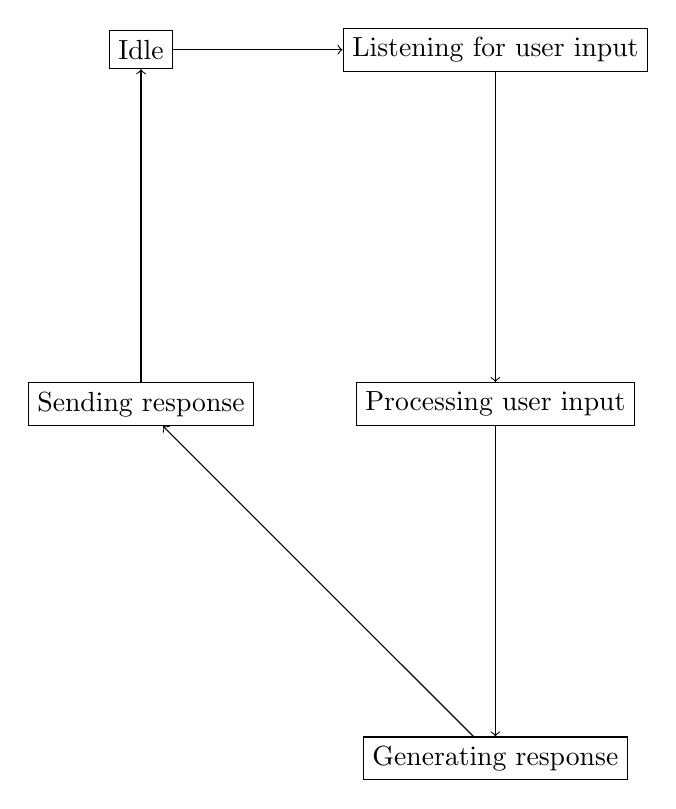
\begin{tikzpicture}[node distance=4.5 cm]
\node[rectangle, draw] (A) {Idle};
\node[rectangle, draw] (B) [right of=A] {Listening for user input};
\node[rectangle, draw] (C) [below of=B] {Processing user input};
\node[rectangle, draw] (D) [below of=C] {Generating response};
\node[rectangle, draw] (E) [left of=C] {Sending response};
\draw [->, =>stealth] (A) -- (B);
\draw [->, =>stealth] (B) -- (C);
\draw [->, =>stealth] (C) -- (D);
\draw [->, =>stealth] (D) -- (E);
\draw [->, =>stealth] (E) -- (A);
\end{tikzpicture}
\caption{Simple state diagram for a bot}
\end{figure}

This state diagram provides a clear visual representation of a generic bot's behavior, allowing developers to easily understand how the program is executing and how it will respond to different inputs. State diagrams are particularly useful for onboarding new developers, as they provide a high-level overview of the program's flow without requiring a deep understanding of the code.


\section{ELF / DWARF}
The ELF (Executable and Linkable Format) is a file format used by many Unix-like operating systems to specify the layout of object files and executables. These files contain a wealth of information about the compiled code, including symbols, debugging information, and other metadata.

One component of ELF files is DWARF (Debugging With Attributed Record Formats), which is a debugging data format that specifies the format of debugging information. DWARF data is embedded in ELF files and can be accessed by debuggers, such as gdb, to provide valuable information about the execution of a program.

DWARF data is organized into structures called DIEs (Debugging Information Entries), which contain tags identifying the type of information they contain. Some common DIE tags include DW\_TAG\_variable for variables, DW\_TAG\_subprogram for functions, and DW\_TAG\_compile\_unit for compilation units. \\

\begin{table}
\centering
\begin{tabular}{|c|c|}
\hline
\textbf{Attribue} & \textbf{Description} \\ \hline
DW\_AT\_name & The name of the subprogram \\ \hline
DW\_AT\_low\_pc & The starting address of the subprogram \\ \hline
DW\_AT\_high\_pc & The ending address of the subprogram \\ \hline
DW\_AT\_decl\_file & The file in which the subprogram is declared \\ \hline
DW\_AT\_decl\_line & The line on which the subprogram is declared \\ \hline
DW\_AT\_prototyped & Specifies whether the subprogram has a prototype \\ \hline
\end{tabular}
\caption{A table of attributes for a DW\_TAG\_subprogram DIE.}
    \label{fig:subprogram_die}
\end{table}

By parsing out these DIE tags, debuggers can access valuable information about the symbols in a program, allowing them to provide useful features such as the ability to inspect and modify variables during execution.

In the context of my live-debugger, Execumap, DWARF data plays a crucial role in my ability to create a state-diagram of the program's execution. By accessing and parsing DWARF data from the recorded trace, I am able to identify the symbols and their relationships in the program.

\section{RR Record and Replay Framework}
The rr record and replay framework is a powerful tool for debugging programs. It allows users to record a program's execution and then replay it at a later time. This allows users to easily and quickly reproduce the conditions that led to a bug. This is particularly useful when debugging rare or timing-sensitive bugs like race conditions where gdb might prevent the bug from ever occuring in the first place.

One key aspect of rr is its focus on capturing nondeterministic input rather than the whole trace \cite{rr-site}. In this case, nondeterministic input are the events that could cause a program's output to vary from run to run. This includes things like syscalls, process-switching timings, or even some non-deterministic instructions. By capturing and replaying these inputs, rr avoids having to walk through and instrument the vast majority of executed instructions. To accomplish this, rr uses a wide variety of tools, including the `ptrace` interface to attach middleware, overwriting the the vDSO (virtual dynamic shared object), limiting a program to a single core, and other more specific techniques. 

To intercept many simple system calls, rr can simply overwrite the vDSO which is a use-space code-segement that the kernel exports for code "that does not necessarily have to run in kernel space" \cite{vdso} However some code directly calls syscalls. As such, "when the tracee makes a system call, RR is notified via a ptrace rap and it tries to rewrite the system-call instruction to call into [their] interception library" \cite[p.~8]{rr}. A diagram of this modification can be seen in figure \ref{fig:subprogram_die}. 

(TODO)
During the replay phase, rr uses this information to replay the system call, allowing the program to execute as if the original system call had been made. This allows rr to accurately reproduce the program's execution, including any system calls that were made. 
(TODO)

\begin{figure}
\centering
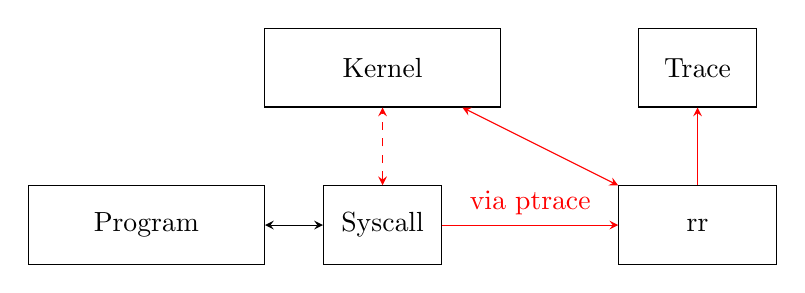
\begin{tikzpicture}

%RR
\node[rectangle, draw, minimum width=2cm, minimum height=1cm] (rr) at (7,-2) {rr};

%Kernel
\node[rectangle, draw, minimum width=3cm, minimum height=1cm] (kernel) at (3,0) {Kernel};

%Program
\node[rectangle, draw, minimum width=3cm, minimum height=1cm] (program) at (0,-2) {Program};

%VDSO
\node[rectangle, draw, minimum width=1.5cm, minimum height=1cm] (syscall) at (3,-2) {Syscall};

%Trace
\node[rectangle, draw, minimum width=1.5cm, minimum height=1cm] (trace) at (7,0) {Trace};

%System Call
\draw[<->, >=stealth] (program) -- (syscall);
\draw[<->, >=stealth, red, dashed] (syscall) -- (kernel);
\draw[<->, >=stealth, red] (rr) -- (kernel);
\draw[->, >=stealth, red] (syscall) -- (rr) node[midway,above ] {via ptrace};
\draw[->, >=stealth, red] (rr) -- (trace);

\end{tikzpicture}
\caption{Diagram showing how rr intercepts calls into the kernel and records them}
\end{figure}
    In order to efficently "continue-backwards", rr utilizes a checkpointing system. The checkpointing system works by \begin{verbatim}fork\end{verbatim}ing the process to cheaply copy the address space \cite[p.~15]{rr}. This is efficient because "fork is (mostly) 'copy-on-write' and is very well optimized on Linux, so creating a checkpoint typically takes less than ten milliseconds." \cite[p.~15]{rr}. This allows rr to quickly and easily restore the program to the state it was in at the time of the checkpoint during the replay phase. Then it can "continue-forwards" until it reaches the desired location.

The default interface to rr is a gdb server using the gdb messaging protocol. However, this is not a performant solution for a programmatic interface that might be doing queries across the entire execution of a program. As such, we developed librr, a Rust library to interact with the C++ internals and provide nice abstractions such as reading registers, writing bytes in memory, setting breakpoints, etc. 

Execumap uses RR (and librr) extensively and would not be possible without them. The ability to gather more information about a programs execution after it happened is has been useful as I am not able to predict all of the locations that a user might want to visit. Similarly, without these tools I would be unable to allow the user to open up the trace to any location within the program's execution.



\chapter{Understanding Code}
Understanding code can be difficult, and blindly building a tool to improve the process is likely to get nowhere. As such, in order to learn how we can help build a tool, we conducted a case study wherein we spent a week studying and understanding a code base while recording our observations. The goal was to use only the codebase itself and no video-lectures or explanations that might not exist for all codebases (especially if they are proprietary). The codebase that we chose was the glibc memory allocator, commonly referred to by its most used function, malloc. The memory allocator uses a wide array of complicated datatypes, intricate macros, and C pointer tricks. The memory allocator also is extremely well documented with comments long expository comments. These comments act as a stand-in for a mentor at a company or someone who knows the codebase well.

In order to tackle this problem, we first conducted a bit of research on tools in this area and were fairly dissapointed. Almost all resources we could find online reccomended the same advice: step through the code with a debugger, write some simple code that interacts with the library to explore its API, keep notes, and just read the source code (with tools provide features like jumping to definitions and collapsing modules). (TODO: src)

\noindent After our study, we arrived at a the following conclusions:
\begin{enumerate}
    \item Malloc is more complicated than we had imagined.
    \item Gdb is perfect for examining a single function execution in high detail, however it fails at helping the programmer easily understand how functions fit together. In order to understand how functions fit together, we set huge numbers of breakpoints and played around with the execution, jumping around and seeing where things took us. This was useful to understand the sections, however we noticed that we had a hard time dealing with the signal to noise ratio of gdb. 
    \item The comments are extremely detailed and any changes that are made to malloc will require careful changes to the documentation that is scattered around the source code. We didn't find any instances of incorrect comments but can easily envision how documentation that is seperate from the implementation could become outdated
    \item Writing everything down is painful and tedious however it was very helpful for our understanding as it allowed us to focus on the high level concepts while also explaining the low level implemenation.
    \item Jumping around the source code with definitions and code collapsing was critical to keep the amount of information in our "working-memory" focused on understanding an individual task.
\end{enumerate}


\chapter{Design}
We spent a significant amount of time designing the user interaction for our application. Initially, we planned to build a gdb plugin that would allow the user to view the state machine graph from the terminal and add annotations directly from the terminal. However, after attempting to write simple gdb plugins, we concluded that it was outside the scope of this project. Therefore, we chose to develop a more GUI-focused application that allows the user to interact with the graph.

To create a responsive and interactive frontend for our application, we decided to split it into a HTTP server backend and a frontend architecture. This decision was not related to the eventual choice of a web-based interface, but rather to simplify the backend. This avoided the need for a message queuing or threadpool system, which would have been necessary in a single unified system to prevent the frontend from freezing whenever the user clicked anything.

The separated networked architecture also enables us to support remote debugging without major ergonomic impacts. This is because the backend and frontend can communicate over the network, allowing us to debug and troubleshoot issues without being in the same physical location as the application.

In addition, splitting the frontend and backend gave us more flexibility in designing the frontend. We were able to focus on creating a user-friendly and intuitive interface without worrying about the underlying logic and functionality of the application.

However, this architecture also has some drawbacks. It increases the overall complexity and overhead of the project, as there are now two separate components that need to be maintained and developed. It also introduces more dependencies for the project, which can potentially cause issues. Overall, while the benefits of a separated architecture are significant, it is important to carefully consider the potential drawbacks before implementing it in a project.

\section{Frontend Platform}
As a Rust developer, I had always been on the lookout for native libraries that would allow me to create robust, efficient, and visually appealing front-end applications. When I stumbled upon Druid, it seemed like the perfect fit.

Druid promised a react-like component-based approach to front-end development, making it easy to modularize and reuse code. Its API was intuitive and well-documented, and it had a growing community of users.

However, as I started using Druid, I quickly realized that it was not as seamless as I had hoped. While the component-based approach was great for building simple, static interfaces, it lacked the ability to easily integrate with other libraries.

For example, I wanted to use a syntax highlighter in my application, but Druid did not have any built-in support for it. I would have had to write my own syntax highlighter from scratch, which was not something I had the time or expertise to do.

I also wanted to include a graph viewer in my application, but again, Druid did not have any built-in support for it. I ended up writing my own graph viewer, but the result was not pretty. It was clunky and difficult to use, and it didn't have the same level of polish as other graph viewers I had seen.

I tried other Rust native libraries like iced and gtk, but they had similar limitations. They were great for building simple interfaces, but they lacked the flexibility and integration capabilities of React.

In the end, I reluctantly fell back to using React for my front-end application. While it was not my ideal choice, it allowed me to quickly and easily integrate with other libraries, and it gave me the ability to create a more polished, user-friendly interface.

\chapter{Graph Simplification}

Once we began generating graphs, we immediately noticed that the graphs were neigh unusable for all but the simplest programs. Generally, these graphs were rendered as giant nests of events where each event had many edges in all different parts of the codebase. 

\section{Synoptic}
The first tool we used to simplify this was a FSM miner, synoptic. One problem that we ran into early on was that the naive way of displaying events was useless for all but the simplest traces. In this case, the naive way is to have one graph node for every event, and to have a edge between two nodes if and only if the target event directly follows the source event. The issue with this 




\section{Modules}
Another technique that was employed to great extent was the development of a module system for events. Modules can act as a namespace for each event. For example, consider two events that indicate the "entry" point of a function. One option is to name the first, func1\_entry and the second func2\_entry. However, this becomes tedious quickly and prohibits any intelligent grouping of events. As such, we create a module system using a similar syntax to many popular programming languages. 

The syntax works by defining a module with a unique name and a single parent. Ex: malloc is a child of glibc, free is also a child of glibc. Then the entry point of free can be specified as free::entry and the entry point of malloc can be specified as malloc::entry. 

This might look like the following in code:

(TODO MAKE THIS A CODE BLOCK)
\begin{verbatim}
// The following metadata sets up the modules used in this example
// [[{type:"module", name:"glibc"}]]
// [[{type:"module", name:"malloc", parent:"glibc"}]]
// [[{type:"module", name:"free", parent:"glibc"}]]

uptr_t malloc(...){
    // Define a start event that gets expanded into glibc::malloc::entry
    // [[{type:"event", name:"malloc::entry"}]]
    ...
}
uptr_t free(...){
    // Define a start event that gets expanded into glibc::free::entry
    // [[{type:"event", name:"free::entry"}]]
    ...
}
\end{verbatim}

TODO image of a graph created by module system

It is best to keep the number of modules to a minimum as otherwise it can create some very ugly graphs, however with a few carefully placed modules, the graph can become much more understandable. You can also click on any module to expand/collapse all of the nodes within it. This can help the viewer start at a much higher level for complicated programs.



\section{Grouping Strictly Sequential Nodes}
The last major technique we used to simplify these graphs was the idea of grouping nodes that are strictly sequential. For this section, we say that nodes A,B are strictly sequential if and only if the only edge out of A is to B, and the only edge into B is from A. Similarly, (A,B,C) is strictly sequential if and only if A and B are strictly sequential, and B and C are also strictly sequential. One of the downfalls of using synoptic for graph simplification is that the final result has many more nodes than the number of edges. By grouping sets of strictly sequential edges, it becomes much easier to understand how nodes relate to each other because it forces graphviz to place multiple sequential steps closer together.


TODO graph on / off


\chapter{Efficient Address Recording}
\label{sec:effaddrrec}

To understand the flow of a program, we need to record the path that it takes. For statically compiled binaries, this is equivalent to recording the locations in memory where the CPU is executing instructions. One way to determine this path is to set "software breakpoints" at various addresses and then continue until the CPU hits one of these breakpoints.

However, when we began our analysis of librr, we quickly noticed that singlestepping and continuing (interrupting the process) incurs a heavy performance penalty. Early measurements indicated overhead on the order of $100 \mu s$ per software breakpoint. This resulted in a ~100-1000x performance penalty depending on the workload. This is unacceptable for anything but the simplest of programs. As a result, we decided to use a more complicated technique called code stomping to force the underlying program to store its location in the program without using software breakpoints.

\section{Naive Implementation}

To have the program record its own location, we created two new memory regions: the address-segment and the trampoline-segment.

The trampoline segment stores code that acts as a recorder for the addresses that are reached. The address-segment acts as the space that the code in the trampoline-segment can use to store the instrumented addresses. To instrument an address, we simply replace the instruction at that address with a jump to an entry in the trampoline-segment.

The address-segment looks like the following:
\subsection{Address-segment diagram}
\begin{drawstack}
  \startframe
  % \cellcom writes something on the right-hand side of a cell.
  \cell{RSP Storage} \cellcom{points to top of stack}
  \cell{...}
  \finishframe{Reserved (40 bytes)}
  \startframe
  \cell{...} \cellcom{}
  \cell{Addr n} \cellcom{top of stack}
  \cell{Addr n-1} \cellcom{}
  \cell{Addr n-2} \cellcom{}
  \cell{...} \cellcom{}
  \cell{Addr 0} \cellcom{base of stack}
  \finishframe{Recorded Addresses Stack}
\end{drawstack}

\subsection{Sample trampoline-segment entry}
\begin{verbatim}
{instruction that was stomped}
XCHG rsp (beginning the address-segment)
PUSH (address of instruction that was skipped)
XCHG rsp (beginning of the address-segment)
JMP (address to go to next instruction in the main program)
\end{verbatim}

\subsection{Considerations}
\begin{enumerate}
    \item This has no protection against overflowing the stack in the address-segment
    \item You can only place trampolines on instructions that are 5+ bytes 
    \item Yon can only place trampolines on instructions that do not alter program flow (for now)
\end{enumerate}


\section{Stack overflow protection}
One problem with this implementation is that it wastes stack space and is risky because if the stack overflows, the user will get a segfault that is difficult to debug. Therefore, we also developed another implementation that includes stack overflow protection. This implementation uses a special byte that is overwritten whenever the stack grows into the reserved space, triggering a software breakpoint and an interrupt that allows the main program to reset the stack.

\noindent Key pieces of information:
\begin{itemize}
    \item No code I write here can increment the x86 retired branch counter as otherwise there will be diversions from the recording. This means that I cannot just compare RSP with some value and then interrupt. 
    \item The INT3 (0xcc) instruction triggers an interrupt that the CPU and kernel use to alert the debugger that a software breakpoint was reached.
    \item The NOP (0x90) instruction is the same size as INT3 (1 byte) 
\end{itemize}
\subsection{Address-segment diagram}
\begin{drawstack}
  \startframe
  % \cellcom writes something on the right-hand side of a cell.
  \cell{RSP Storage} \cellcom{points to top of stack}
  \cell{RAX Storage} \cellcom{}
  \cell{...}
    \cell{Overflow Detection Byte} \cellcom{intial: 0x90 (NOP)}
    \finishframe{Reserved (40 bytes)}
  \startframe
  \cell{...} \cellcom{}
    \cell{0xcccccccc} \cellcom{Canary to trip overflow byte}
  \cell{Addr n} \cellcom{top of stack}
  \cell{Addr n-1} \cellcom{}
  \cell{Addr n-2} \cellcom{}
  \cell{...} \cellcom{}
  \cell{Addr 0} \cellcom{base of stack}
  \finishframe{Recorded Addresses Stack}
\end{drawstack}


\subsection{Sample trampoline-segment entry}

\begin{verbatim}
{instruction that was stomped}
XCHG rsp (beginning of the address-segment)
XCHG rax (beginning of the address-segment + 8)
PUSH (address of instruction that was skipped)
PUSH 0xcccccccc
POP  <- subtracts from RSP without clearing the memory in front of it 
MOV AL (overflow detection byte) 
MOV (RIP+1) AL
NOP  <- instruction that will be overwritten by overflow detection byte
XCHG rsp (beginning of the address-segment)
XCHG rax (beginning of the address-segment + 8)
JMP (address to go to next instruction in the main program)
\end{verbatim}


\subsection{Considerations}
\begin{enumerate}
    \item This requires the trampoline segments to have more than twice as many instructions
    \item You can only place trampolines on instructions that are 5+ bytes 
    \item Yon can only place trampolines on instructions that do not alter program flow (for now)
\end{enumerate}
\section{Final Implementation}
After some experimentation, we determined that it was easiest to simply use the naive implementation and give the address-segment a large (256Mib) buffer. We then clear this stack every time a new "frametime" event triggers, which happens on average every $40,000,000$ instructions \cite[Scheduler.h:72]{librr-src}. This allows us to process on the order of $10^9$ instructions per second (at peak thoretical throughput with no saving overhread). We have not conducted in depth benchmarks on this because this system has completelly eliminated the problem of address recording speed. 




% Describe Synoptic

\chapter{Conclusions and Future Work}
In this report, we presented Explorant, a novel onboarding and code exploration tool. Explorant was designed to improve many of the issues that we encountered in our case study of \texttt{malloc} and we think that it has succeeded at its mission and more. 

As time goes on, we hope that Explorant will continue to develop and address some of its main weaknesses. While many of the limitations brought up in section \ref{sec:design-limitations} cannot be fixed (like JIT support), a number of them can. The areas we think are ripe for future work are:
\begin{itemize}
    \item A user study evaluating the effectiveness of this tool and its usefulness
\item The ability to compare multiple traces at once and build a combined graph from all of them.
\item The ability to drag around nodes and add custom edges and labels within the graph so that the graphs can serve as official documentation
\item Fixing difficultiies with long running executions using complex function call heatmaps or simply limiting the execution to a smaller range (perhaps both) 
\item Automaic segmentation of events based off of filesystem hierarchies rather than modules. We think this would be particularly useful for codebases with a large number of disjoint files.
\item Possible automatic event definition based on some criteria from the trace that contain the fewest nodes but capture the most important flow paths. 
\end{itemize}

We strongly believe this tool can serve as a critical resource not only for new developers understanding a codebase, but also for senior engineers who can add Explorant annotations and have the junior engineers explore on their own. We will continue supporting Explorant and we hope others embrace and extend our work to realize the next generation of code exploration.



\newpage % Start new page
\begin{appendices}

\section{Appendix A Title}
\label{appendix:appendix_a_label}

Input materials for Appendix A. Works the same as regular text, just do not include captions or labels on any tables or figures. Appendices can be referenced in text the same way you reference figures or tables, using the label. 

\newpage

\section{Appendix B Title}
\label{appendix:appendix_b_label}

Input materials for Appendix B

\end{appendices}

\newpage % Start new page
\end{doublespacing} % Return to single spacing
\addcontentsline{toc}{section}{References} % Add the 'References' section to the table of contents
\bibliographystyle{IEEEtran} % Set the bibliography style
\bibliography{bibliography.bib} % Generate a bibliography from the .bib file with all of the references
\end{document}
